After the discovery of the Higgs boson~\cite{HIGG-2012-27,CMS-HIG-12-028}, the scrutiny of the electroweak symmetry breaking (EWSB) becomes a main focus at the LHC. In addition to direct measurements of Higgs boson properties, the study of massive vector-boson scattering (VBS) offers another key avenue to probe the EWSB~\cite{Lee:1977yc,Chanowitz:1985hj,Szleper:2014xxa}. In the Standard Model (SM), the Higgs boson acts rigorously to prevent longitudinal VBS amplitudes from violating unitarity at the \TeV~scale~\cite{Lee:1977yc}; therefore, the study of high-energy behaviours of VBS is crucial to understand the nature of the EWSB. Many new physics scenarios, such as Supersymmetry and Little Higgs models~\cite{ArkaniHamed:2002qy}, offer alternative EWSB mechanisms, which can manifest themselves as appearance of heavy particles or modifications of Higgs couplings in the accessible energy regime.
These new phenomena could manifest themselves in rises of amplitudes or resonant structures in the TeV range and thereby alter the way of delicate cancellations at high energies.

While no VBS processes were established prior to the LHC era, the LHC provides an unprecedented opportunity to study them, owing to its high collision energies and luminosities. At the LHC, VBS is typically produced as two vector bosons radiated from initial-state quarks and then scattering into another pair of vector bosons. The detector signature of VBS contains decay products of the pair of outgoing bosons and a pair of hadronic jets, hereafter denoted as $VVjj$. The most promising channel to measure VBS is therefore the electroweak (EW) production of $VVjj$ (EW $VVjj$), which has no quantum chromodynamics (QCD) vertices at leading order (LO).
The QCD production of $VVjj$ contains two QCD vertices at the lowest order (denoted as QCD $VVjj$ processes) and constitutes an irreducible background to the searches for EW $VVjj$ production. The characteristics of EW $VVjj$ production include a large separation in rapidity between the two jets (\dyjj) as well as a significant invariant mass of the jet pair (\mjj), which are often utilized to improve the signal-to-background ratio. 

Among all the EW $VVjj$ processes with massive bosons, the EW $W^{\pm}W^{\pm}jj$ and $WZjj$ processes have been observed~\cite{Aaboud:2019nmv,Aaboud:2018ddq,Sirunyan:2017ret} using LHC Run 2 data, and no obvious deviations from the SM predictions were found. The EW $ZZjj$ production was searched for by the CMS collaboration using 36.1 \ifb~of 13 \TeV~$pp$ collision data, but no evidence was found~\cite{Sirunyan:2017fvv}. This type of rare processes has a fiducial cross-section of the order of $O(0.1)$ fb in the final states where both $Z$ bosons decay leptonically.
Despite the small rate, EW $ZZjj$ production offers a clean and competitive channel to study EWSB physics. Observation of EW $ZZjj$ production is another milestone for the physics program at the LHC. Figure~\ref{fig:diagram} depicts the typical diagrams for both the EW and QCD $ZZjj$ processes. 

This talk reports on the observation of EW $ZZjj$ (including contribution from $\gamma^*$) production by the ATLAS experiment, using the complete set of 13 \TeV~$pp$ collision data taken in LHC Run 2. The search is performed in two final states where both $Z$ bosons decay leptonically: four charged leptons with two jets (\lllljj), and two charged leptons, two neutrinos and two jets (\llvvjj).
Event selections are optimized to suppress reducible backgrounds, and fiducial cross-sections for the inclusive production of the EW and QCD processes are reported separately in individual channels.
The $ZZjj$ production involving intermediate $\tau$-leptons from $Z$ decays is considered as signal but has a negligible contribution to the selected event sample. Reducible backgrounds give minor contributions in the \lllljj channel.
In the \llvvjj channel, large missing transverse momentum (\met) is required to suppress the background from \Zjet events; other major backgrounds are the production of $WWjj$, $WZjj$ and \ttbar.
To enhance the separation between the EW signal and the main backgrounds, multivariate discriminants (MDs) are trained from event kinematic information using simulated samples.
The MD distributions are fitted simultaneously in the two channels to evaluate the contribution from EW processes.


\begin{figure}[!htbp]
\begin{center}
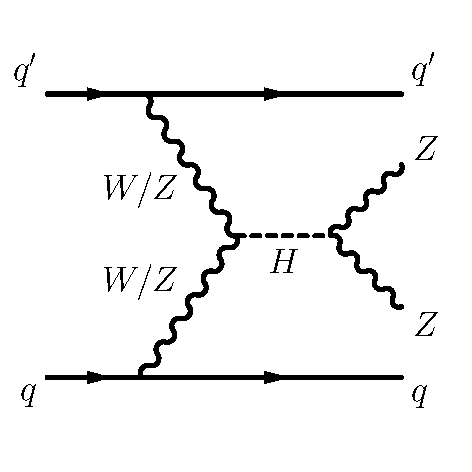
\includegraphics[width=0.22\textwidth]{figures/diagram/diagram-EWZZjj-Schn-Higgs.pdf}
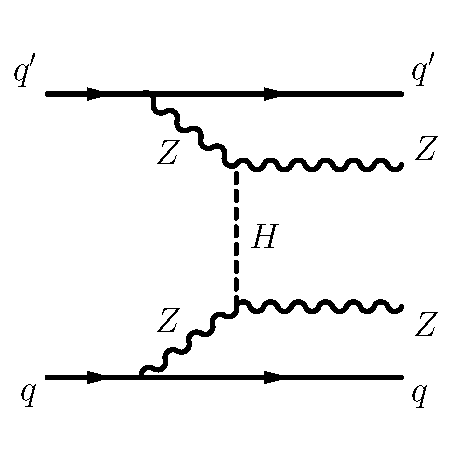
\includegraphics[width=0.22\textwidth]{figures/diagram/diagram-EWZZjj-Tchn-Higgs.pdf}
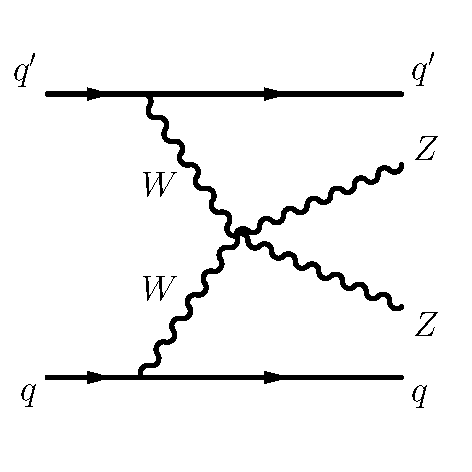
\includegraphics[width=0.22\textwidth]{figures/diagram/diagram-EWZZjj-QGC.pdf}
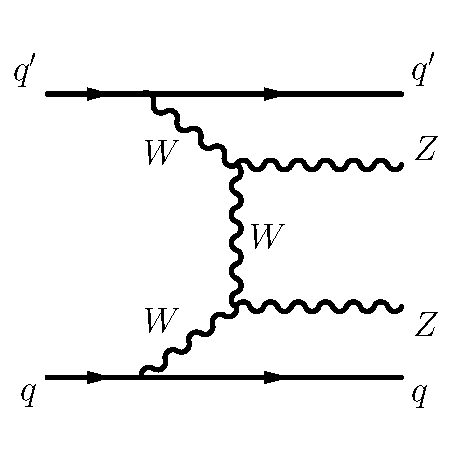
\includegraphics[width=0.22\textwidth]{figures/diagram/diagram-EWZZjj-TGC.pdf}\\
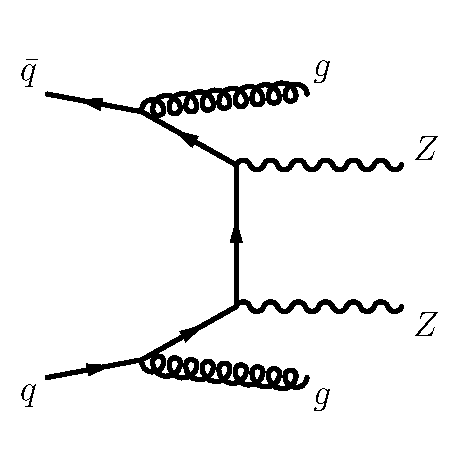
\includegraphics[width=0.22\textwidth]{figures/diagram/diagram-QCDZZjj-qq.pdf}
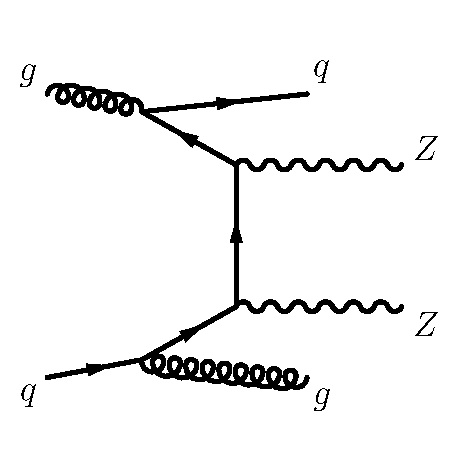
\includegraphics[width=0.22\textwidth]{figures/diagram/diagram-QCDZZjj-qg.pdf}
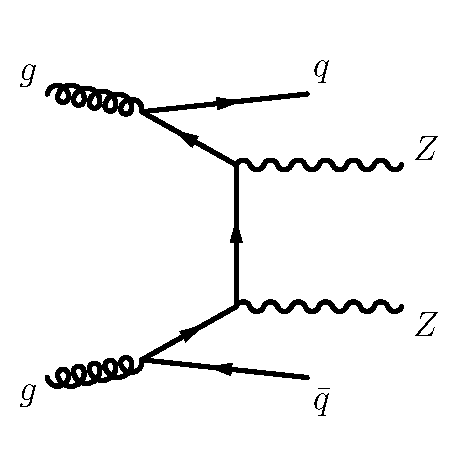
\includegraphics[width=0.22\textwidth]{figures/diagram/diagram-QCDZZjj-gg.pdf}
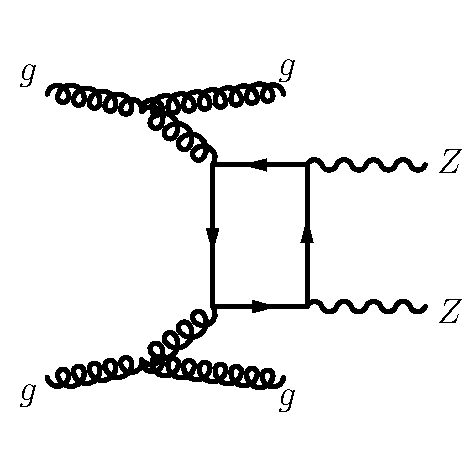
\includegraphics[width=0.22\textwidth]{figures/diagram/diagram-QCDZZjj-box.pdf}\\
\end{center}
\caption{Typical diagrams for the production of $ZZjj$, including the relevant EW VBS diagrams (first row) and QCD diagrams (second row).}
\label{fig:diagram}
\end{figure}
